\section{Relation between odds and SNRs}\label{app:oddratios}

It is interesting to look at how we might expect odds values (ratios of evidences) to vary with signal-to-noise ratio (SNR) \citep[also
see similar discussions in][]{MaxCWpolariations}. We will take the simple case of two Gaussian
datasets both of the same length ($N = 100$) and standard deviation, $\sigma$. Both datasets contains a mean offset of $\mu_h = 5$, and we are concerned with a
search over the mean parameter. We want to calculate two things: the odds for a mean offset versus the data being Gaussian noise with a known mean of zero; and,
the odds for both datasets containing the same mean offset (a coherent signal) versus them containing two independent mean offsets (an incoherent signal). We can
try and work out what to expect using approximations, and then see if that's actually the case when calculating the values analytically.

To set up the situation, we have the two datasets $d_1$ and $d_2$, which have likelihoods given by
\begin{equation}
 p(d_j|\mu,M,I) = \left(\frac{1}{2\pi\sigma^2}\right)^{(N/2)} \exp{\left(-\frac{\sum_i^N (d_{j,i}-\mu_i)^2}{2\sigma^2}\right)},
\end{equation}
and priors on $\mu$ given by $p(\mu|M,I)$, which we will take as constant (i.e.\ a flat prior). We will also use the fact that $d_{j,i} = \mu_t + n_{j,i}$
where $n_{j,i}$ is a value drawn from a Gaussian distribution of zero mean and standard deviation $\sigma$, and $\mu_t$ is the true offset.

To re-cap from earlier in this paper, the evidence is given by
\begin{equation}
\mathcal{Z}_M = \int_{\mu_{\text{min}}}^{\mu_{\text{max}}} p(d|\mu, M, I) p(\mu|M,I) {\text{d}\mu}
\end{equation}
for hypothesis $M$.

\subsection{Coherent signal vs.\ noise odds}

For large SNRs the relation between signal ($S$) versus noise ($N$) evidence odds for Gaussian noise is well known, but we'll write it out explicitly here.
Formally, for our two data steams, we have
\begin{equation}
 \mathcal{O}_{\text{S}/\text{N}} = \frac{\mathcal{Z}_{S}}{\mathcal{Z}_{N}} = (2\pi\sigma^2)^{-N} \frac{p(\mu)}{\mathcal{Z}_{N}} \int_{\mu_{\text{min}}}^{\mu_{\text{max}}} p(d_1|\mu,I) p(d_2|\mu,I) {\text{d}\mu}.
\end{equation}
For high SNR signals the we find that
\begin{equation}
\int_{\mu_{\text{min}}}^{\mu_{\text{max}}} p(d|\mu,M,I) \text{d}\mu \approx p(d|\mu=\mu_{t/\text{ML}},M,I) \left(\frac{2\pi\sigma^2}{N} \right)^{1/2},
\end{equation}
where $p(d|\mu=\mu_{t/\text{ML}},M,I)$ is the likelihood at the true/maximum likelihood value of $\mu$. This value, for the joint datasets, can be seen to be
\begin{equation}
p(\{d\}|\mu=\mu_{t/\text{ML}},M,I) = \left(\frac{1}{2\pi\sigma^2}\right)^{N} \exp{\left(-\frac{1}{2\sigma^2}\sum_i^N \left[(d_{1,i} - \mu_t)^2 + (d_{2,i} - \mu_t)^2 \right]\right)},
\end{equation}
which in turn (with $d_{j,i} = \mu_t + n_{j,i}$) becomes
\begin{align}
p(\{d\}|\mu=\mu_{t/\text{ML}}, M, I) &= \left(\frac{1}{2\pi\sigma^2}\right)^{N} \exp{\left(-\frac{1}{2\sigma^2}\sum_i^N \left[ n_{1,i}^2 + n_{2,i}^2 \right]\right)} \nonumber \\
&\approx \left(\frac{1}{2\pi\sigma^2}\right)^{N} \exp{(-N)},
\end{align}
where we have used $\sum_i^N n_i^2/\sigma^2 \approx N \pm \sqrt{N}$. Similarly, we have the noise evidence
\begin{align}
\mathcal{Z}_N &= \left(\frac{1}{2\pi\sigma^2}\right)^{N} \exp{\left(-\frac{1}{2\sigma^2}\sum_i^N \left[2\mu_t^2 + (n_{1,i}^2 + n_{2,i}^2) - 2\mu_t(n_{1,i} + n_{2,i}) \right] \right)} \nonumber \\
&\approx 
\left(\frac{1}{2\pi\sigma^2}\right)^{N}\exp{\left(-N - \sum_i^N \frac{\mu_t^2}{\sigma^2} \right)},
\end{align}
where we use the approximation that $\sum_i^N \mu_t n_{j,i} \approx 0$. So, the odds becomes
\begin{equation}
\mathcal{O}_{\text{S}/\text{N}} \approx \left(\frac{2\pi\sigma^2}{N} \right)^{1/2}p(\mu|M,I)\exp{\left(\sum_i^N \frac{\mu_t^2}{\sigma^2}\right)},
\end{equation}
where we can also say that the single dataset SNR is defined as $\rho^2 = \sum_i^N \mu_t^2/\sigma^2 = N\left(\mu_t/\sigma\right)^2$, and in this case
$\rho_{\text{coh}} = \sqrt{2}\rho$, and we can see that if we take the natural logarithm of this that
\begin{equation}
\ln{\mathcal{O}_{\text{S}/\text{N}}} = \ln{\left(p(\mu|M,I)\right)} + \frac{1}{2}\ln{\left(\frac{2\pi\sigma^2}{N}\right)} + \frac{1}{2}\rho_{\text{coh}}^2.
\end{equation}
We see here that the log odds is proportional to $\rho^2$, with a minor influence from the $\ln{\left(2\pi\sigma^2/N\right)}$ term which is roughly equivalent
to $\ln{\left(2\pi\rho^{-2}\right)}$. Empirically (and probably with some mathematical justification that can be derived) this approximation seems to give the
median odds value on random realisations of noise, even down to low SNR (see Figure~\ref{fig:approx_odds}).

\subsection{Coherent signal vs.\ incoherent signal}

We can define a coherent signal versus incoherent signal odds ratio as
\begin{equation}
\mathcal{O}_{\text{S}/\text{I}_{\text{simple}}} = \frac{\mathcal{Z}_{\text{coh}}}{\mathcal{Z}_{\text{incoh}}} = \frac{\mathcal{Z}_{\{d\}}}{\mathcal{Z}_{d_1}\mathcal{Z}_{d_2}},
\end{equation}
where $\mathcal{Z}_{\{d\}}$, $\mathcal{Z}_{d_1}$, and $\mathcal{Z}_{d_2}$, are the evidences for a signal in the full dataset, and two individual
datasets (this is equivalent to Equation~\ref{eq:cohvincoh1}). Using the same approximations as above, we find that
\begin{equation}
\mathcal{O}_{\text{S}/\text{I}_{\text{simple}}} \approx \frac{1}{2\sqrt{\pi}}\frac{1}{p(\mu|M,I)}\frac{\sqrt{N}}{\sigma}.
\end{equation}
In this we see that there is the Occam factor of $1/p(\mu|M,I)$ accounting for the fact that the incoherent model has an extra parameter. We also see that this is
proportional to $\sqrt{N}/\sigma$ which is roughly equivalent to $\rho$.

So we see that for the coherent signal versus noise odds roughly scales with $e^{\rho^2}$, whilst the coherent signal versus incoherent signal odds roughly scales with
$\rho$, i.e.\ its scaling is a lot shallower. Empirically (and probably with some mathematical justification that can be derived) this approximation seems to give the
maximum odds value on random realisations of noise down to low SNR (see Figure~\ref{fig:approx_odds}).

In Figure~\ref{fig:approx_odds} we see how these two approximations compare to analytical calculations of the odds values as the SNR changes. For a range of SNRs
we created multiple realisations of two dataset of Gaussian random noise (with SNR altered by altering the standard deviation of the noise) with a given
mean offset. In each case we have analytically calculated the evidences for a coherent $\mu$ for both datasets, and independent $\mu\text{s}$ in both datasets.
These are then compared to the approximations above. In this case we have purposely chosen a prior on $\mu$ such that the distributions of odds values for
$\mathcal{O}_{\text{S}/\text{I}_{\text{simple}}}$ and $\mathcal{O}_{\text{S}/\text{N}}$ cross, which is similar to the case we observed in our actual analysis shown in \S\ref{sec:simsignal}.

\begin{figure}[!phtb]
\begin{center}
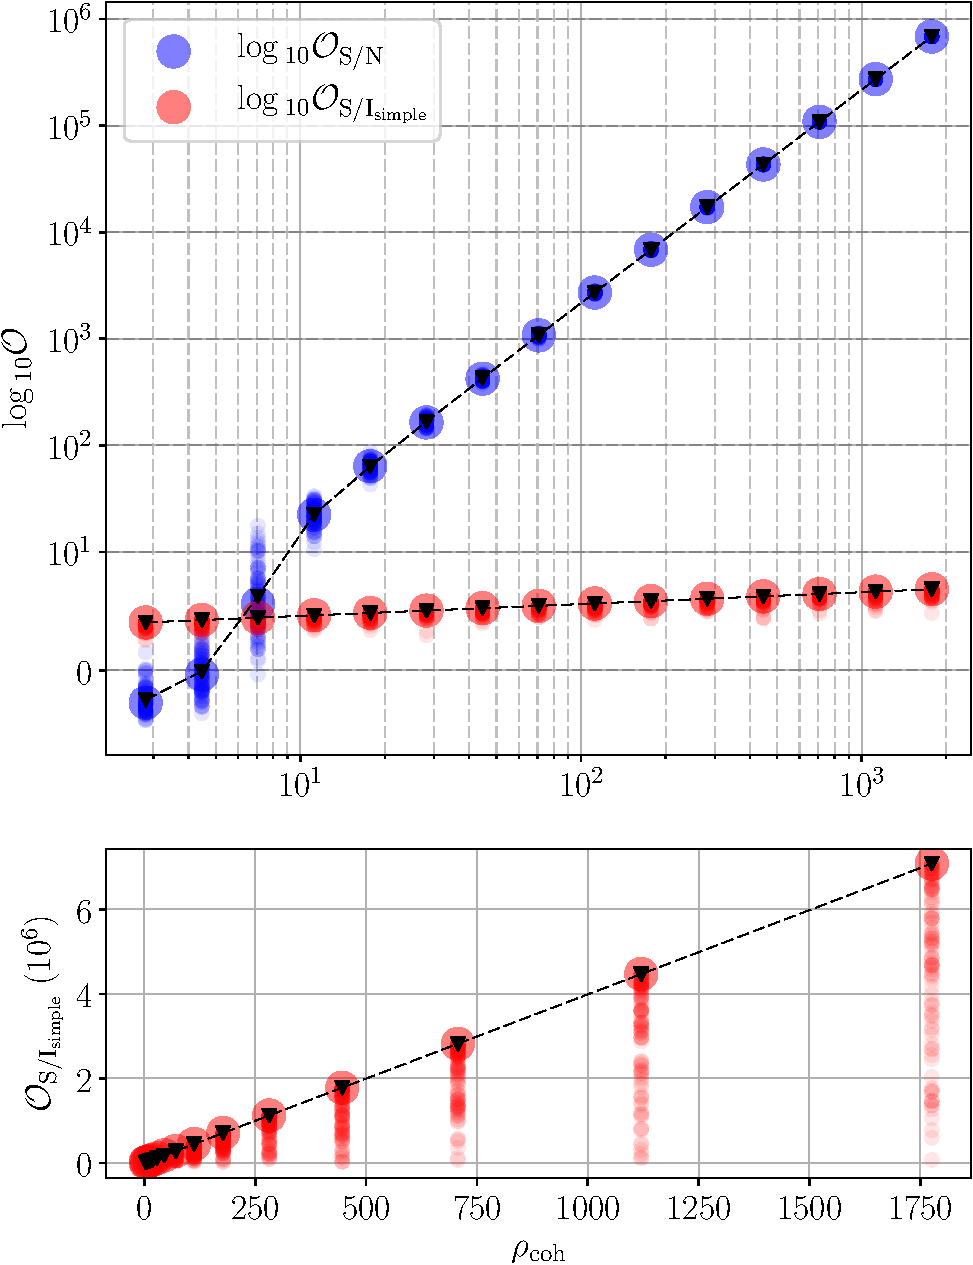
\includegraphics[width=0.5\textwidth]{./figures/appendix4/approx_odds}
\caption{ \protect\label{fig:approx_odds}
The upper plot shows coherent signal-to-noise ratio ($\rho_{\text{coh}}$) versus the logarithm of odds for
two different cases: coherent signal versus Gaussian noise $\mathcal{O}_{\text{S}}/{\text{N}}$ and coherent signal versus
incoherent signal $\mathcal{O}_{\text{S}/\text{I}_{\text{simple}}}$. In both cases, and for each $\rho_{\text{coh}}$, there are values for
100 realisations of noise, with the median and maximum values, for $\mathcal{O}_{\text{S}}/{\text{N}}$ and $\mathcal{O}^S_I$
respectively, highlighted with larger points. Overplotted are the approximate values expected for these two
odds. The lower plot just shows $\mathcal{O}^S_I$ to make its relation to $\rho_{\text{coh}}$ more obvious.
}
\end{center}
\end{figure}
